\documentclass[twoside,10pt]{article}
\usepackage{shlists}
\usepackage[applemac]{inputenc}
\usepackage[spanish]{babel}
\usepackage[T1]{fontenc}


\usepackage{multicol}
\usepackage{picinpar}

\usepackage{url}
\newcommand{\surl}[1]{{\small\url{#1}}}

\newcounter{vol}
\newcounter{num}
\newcounter{anyo}
\setcounter{vol}{9}
\setcounter{num}{2}
\setcounter{anyo}{2016}
\newcommand{\mes}{Mayo}
\usepackage{revisionNLcol}


\title{\ \\ Docencia 2.0\\ \large Juan Juli\'{a}n Merelo, Fernando Tricas}
\author{\LARGE Dise�ando un proyecto}

\date{}

\AutTit{Docencia 2.0}

\begin{document}
\addtocounter{page}{2}

\maketitle
\vspace*{-5ex}

\begin{multicols}{2}
 	
%--------------------------
\noindent\rule{86mm}{1pt}
\vspace{1ex} {\small{\begin{window}[0,r,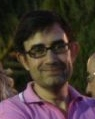
\includegraphics[width = 27mm]{JJM.jpg},] 
\noindent\emph{JJ Merelo} es catedr\'{a}tico de Universidad
en el \'area de Arquitectura y Tecnolog\'{\i}a de Computadores, y
actualmente director de la Oficina de Software Libre de la UGR.
Mantiene un blog desde el a\~no 2002, y lo ha utilizado en clase desde
el a\~no 2004; tambi\'en wikis, agregadores y repositorios de c\'odigo
como herramientas docente. \'{U}ltimamente le ha dado por el \textsl{flipped
learning}, de lo que se informar\'{a} debidamente en esta columna.
\end{window}}}

\medskip

{\small{\begin{window}[0,r,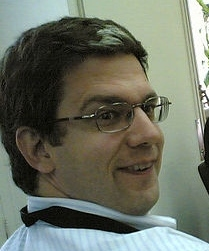
\includegraphics[width = 27 mm]{FTricas1.jpg},]
		\noindent \emph{Fernando Tricas Garc\'{\i}a} es profesor
		titular de Lenguajes y Sistemas Inform\'{a}ticos del Departamento
		de Inform\'{a}tica e Ingenier\'{\i}a de Sistemas de la Universidad de
		Zaragoza.  Empez\'{o} a estudiar la blogosfera casi cuando a\'{u}n no
		exist\'{\i}a (all\'{a} por el a\~{n}o 2002) y a tratar de integrarla en los
		cursos y tareas docentes un poco despu\'{e}s.  Ha impartido
		numerosas charlas relacionadas con el tema de la Web 2.0, 
		internet y universidad,\ldots\ 
		Es actualmente Vicerrector de Tecnolog\'{\i}as de la Informaci\'{o}n y
de la Comunicaci\'{o}n.   
		\end{window}}}
%-------------------------------------------------

		



\noindent 
\bigskip

\noindent\emph{Todas las columnas de la serie Docencia 2.0
pueden descargarse en formato LaTeX desde
\surl{https://github.com/ReVision-Docencia-20/Columnas}}

\noindent\rule{90mm}{1pt}

{\small \noindent\copyright 2016 JJ. Merelo, F. Tricas. Este art\'{\i}culo es de acceso libre distribuido bajo los t\'{e}rminos
de la Licencia Creative Commons de Atribuci\'{o}n, que permite copiar,
distribuir y comunicar p\'{u}blicamente la obra en cualquier medio, s\'{o}lido
o electr\'{o}nico, siempre que se acrediten a los autores y fuentes
originales}

\end{multicols}
\end{document}
